\newcommand{\equadiff}{/home/robin/ENSEIGN/Cours/MathBiologie/L3-ENS-Math1/Exercices/EquaDiff}

%-------------------------------------------------------------------------------
\subsection{Calcul différentiel}
%-------------------------------------------------------------------------------

%-------------------------------------------------------------------------------
\subsubsection{Application linéaire tangente à une forme quadratique} 
%-------------------------------------------------------------------------------

On considère une matrice $A \in \Mcal_n$ symétrique, un vecteur $v \in \Rbb^n$ et la fonction 
$$
\begin{array}{rlll}
  f : & \Rbb^n & \mapsto & \Rbb \\
  & x & \to & f(x) = x^\top A x + v^\top x.
\end{array}
$$

\begin{enumerate}
  \item Montrer qu'il existe un vecteur $g(x) \in \Rbb^n$, qu'on précisera, tel que l'application linéaire tangente à $f$ en $x$ s'écrit
  $$
  \begin{array}{rlll}
    D_xf : & \Rbb^n & \mapsto & \Rbb^n \\
    & h & \to & D_xf(h) = g(x)^\top h.
  \end{array}
  $$
  \solution{On écrit
  \begin{align*}
    f(x+h) 
    & = (x+h)^\top A (x+h) + v^\top (x+h)
    = f(x) + x^\top A h + h^\top A x + h^\top A h + v^\top h \\
    & = f(x) + (2 x^\top A + v^\top) h + h^\top A h
  \end{align*}
  puisque $x^\top A h = h^\top A x$. On remarque alors que $h^\top A h = o(\|h\|)$ pour conclure que, puisque $A$ est symétrique, l'application linéaire tangent $D_x f$ s'écrit bien
  $$
  D_xf(h) = g(x)^\top h
  \qquad \text{avec} \quad
  g(x) = 2 A x + v.
  $$}
  \item En supposant que $A$ est inversible, déterminer le point stationnaire $x^*$ où $g(x)$ s'annule.
  \solution{En supposant $A$ inversible, on a
  $$
  g(x^*) = 0
  \qquad \Leftrightarrow \qquad
  2 A x^* + v = 0
  \qquad \Leftrightarrow \qquad
  x^* = - \frac12 A^{-1} v.
  $$}
  \item Donner une condition sur$A$ pour que $A$ soit un minimum local. (On pourra calculer la matrice hessienne de $A$.)
  \solution{La matrice hessienne de l'application $f$ en tout point $x$ vaut $H_x = 2 A$ (il suffit de déterminer l'application linéaire tangente à $g(x)$).
  $x^*$ est donc un minimum ssi $A$ est strictement définie négative}
  \item Discuter l'utilité de l'hypothèse selon laquelle $A$ est symétrique.
  \solution{On peut décomposer $A$ en ses parties symétrique $S$ et anti-symétrique $T$ : 
  $$
  S = \frac12(A + A^\top), \qquad 
  T = \frac12(A - A^\top), \qquad 
  \Rightarrow \quad
  A = S + T
  $$
  et remarquer que
  $$
  f(x) 
  = x^\top A x + v^\top x
  = x^\top S x + \frac12 \underset{=0}{\underbrace{(x^\top A x - x^\top A^\top x)}} + v^\top x,  
  $$
  c'est-à-dire que seulle la partie symétrique de $A$ contribue à la fonction Ode $f$.}
\end{enumerate}




%-------------------------------------------------------------------------------
\subsection{Systèmes dynamiques en dimension 1}
%-------------------------------------------------------------------------------

%-------------------------------------------------------------------------------
\subsubsection{L3 Bio SU : TD2, exercice 1 \todo{}} 
%-------------------------------------------------------------------------------

\todo{Voir L3 Bio SU : TD2, exercice 1}


%-------------------------------------------------------------------------------
\subsubsection{Système différentiel d'ordre trois} 
%-------------------------------------------------------------------------------

On considère l'équation différentielle ordinaire non-linéaire
\begin{equation} \label{eq:L3BioSUTD2E2}
\dot x = f(x) = -x^3 + 7x^2 - 14x + 8.
\end{equation}
% dans laquelle $x$ désigne la concentration d'un métabolite : \eqref{eq:L3BioSUTD2E2} modélisant l'ensemble des réactions biochimiques impliquées dans la production/dégradation de ce métabolite.

\begin{enumerate}
  \item Déterminer l'ensemble des points stationnaires de \eqref{eq:L3BioSUTD2E2}.
  \solution{On cherche les raçines de $f(x)$. 1 est une racine évidente, et, en déterminant les raçines de $x^2 - 6x + 8$, on voit que $f(x)$ se factorise en
  \begin{align*}
    f(x) & = (x-1) (x^2 - 6x + 8) = (x-1) (x - 2) (x - 4). 
  \end{align*}
  Les points stationnaires sont donc $x^*_1 = 1$, $x^*_2 = 2$ et $x^*_3 = 4$.}
  \item \'Etudier la stabilité de chacun de ces points stationnaires.
  \solution{On calcule
  $$
  f'(x) = -3 x^2 + 14x -15
  $$
  et on conclue 
  \begin{align*}
    f'(x^*_1) & = -3 < 0 & \Rightarrow \quad x^*_1 & = 1 \text{ est stable}, \\ 
    f'(x^*_2) & = + 2 > 0 & \Rightarrow \quad x^*_2 & = 2 \text{ est instable}, \\ 
    f'(x^*_3) & = -6 < 0 & \Rightarrow \quad x^*_3 & = 4 \text{ est stable}. 
  \end{align*}}
  \item Tracer le diagramme de stabilité du système.
  \solution{$$
  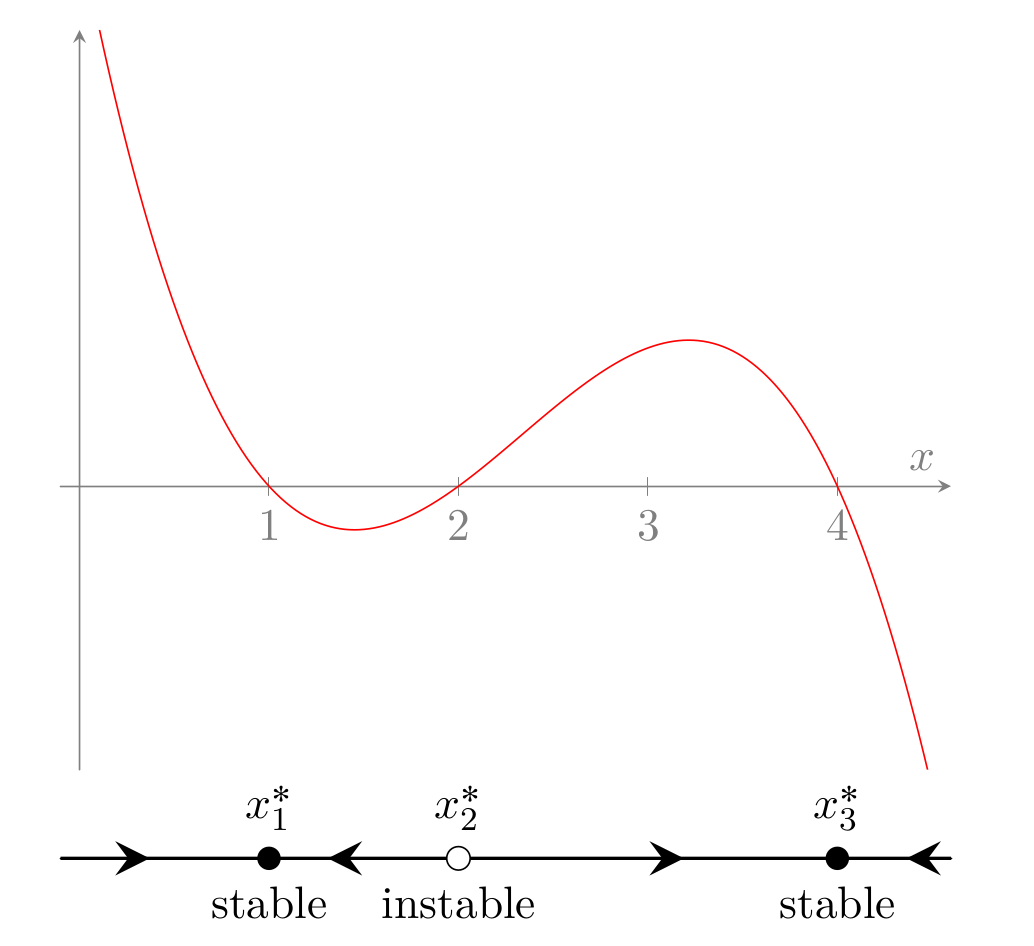
\includegraphics[width=.4\textwidth]{L3bioSU-TD2exo2}
  $$}
  \item D'un point de vue du comportement du système, quels sont les rôles respectifs de chacun des points stationnaires.
  \solution{
  \begin{itemize}
   \item $x^*_1$ et $x^*_3$ sont des équilibre stables et attracteurs vers lesquels le système tend. On perle de bistabilité.
   \item $x^*_2$ est le point critique (stationnaire mais répulsif) : la position de $x(0$ par rapport à $x^*_2$ détermine l'état final du système.
  \end{itemize}}
\end{enumerate}


%-------------------------------------------------------------------------------
\subsubsection{Modèle cubique}
%-------------------------------------------------------------------------------

% [Exercice 2, TD2, L2 Bio SU]

\exemple{
  On considère le système
  $$
  \dot y = - y^3 + 7 y^2 - 14 y + 8.
  $$
  Ses points stationnaires sont les racines du polynôme $P(y) = - y^3 + 7 y^2 - 14 y + 8$, donc $y_1 = 1$ fait partie, donc
  $$
  P(y) = (y-1) (-y^2 + 6y + 8),
  $$
  et les deux racines de $-y^2 + 6y + 8$ sont $2$ et $4$. Les points stationnaires du système sont donc 
  $$
  y_1 = 1, \qquad y_2 = 2, \qquad y_3 = 4.
  $$
  Leur stabilité est donné par la dérivée de $P$:
  $$
  P'(y) = -3y^2 + 14 y - 14,
  $$
  soit
  $$
  P'(y_1) = -3, \qquad P'(y_2) = 2, \qquad P'(y_3) = -6.
  $$
  $y_1$ et $y_3$ sont donc des équilibres stables, et $y_2$ un équilibre instable.
  $$
  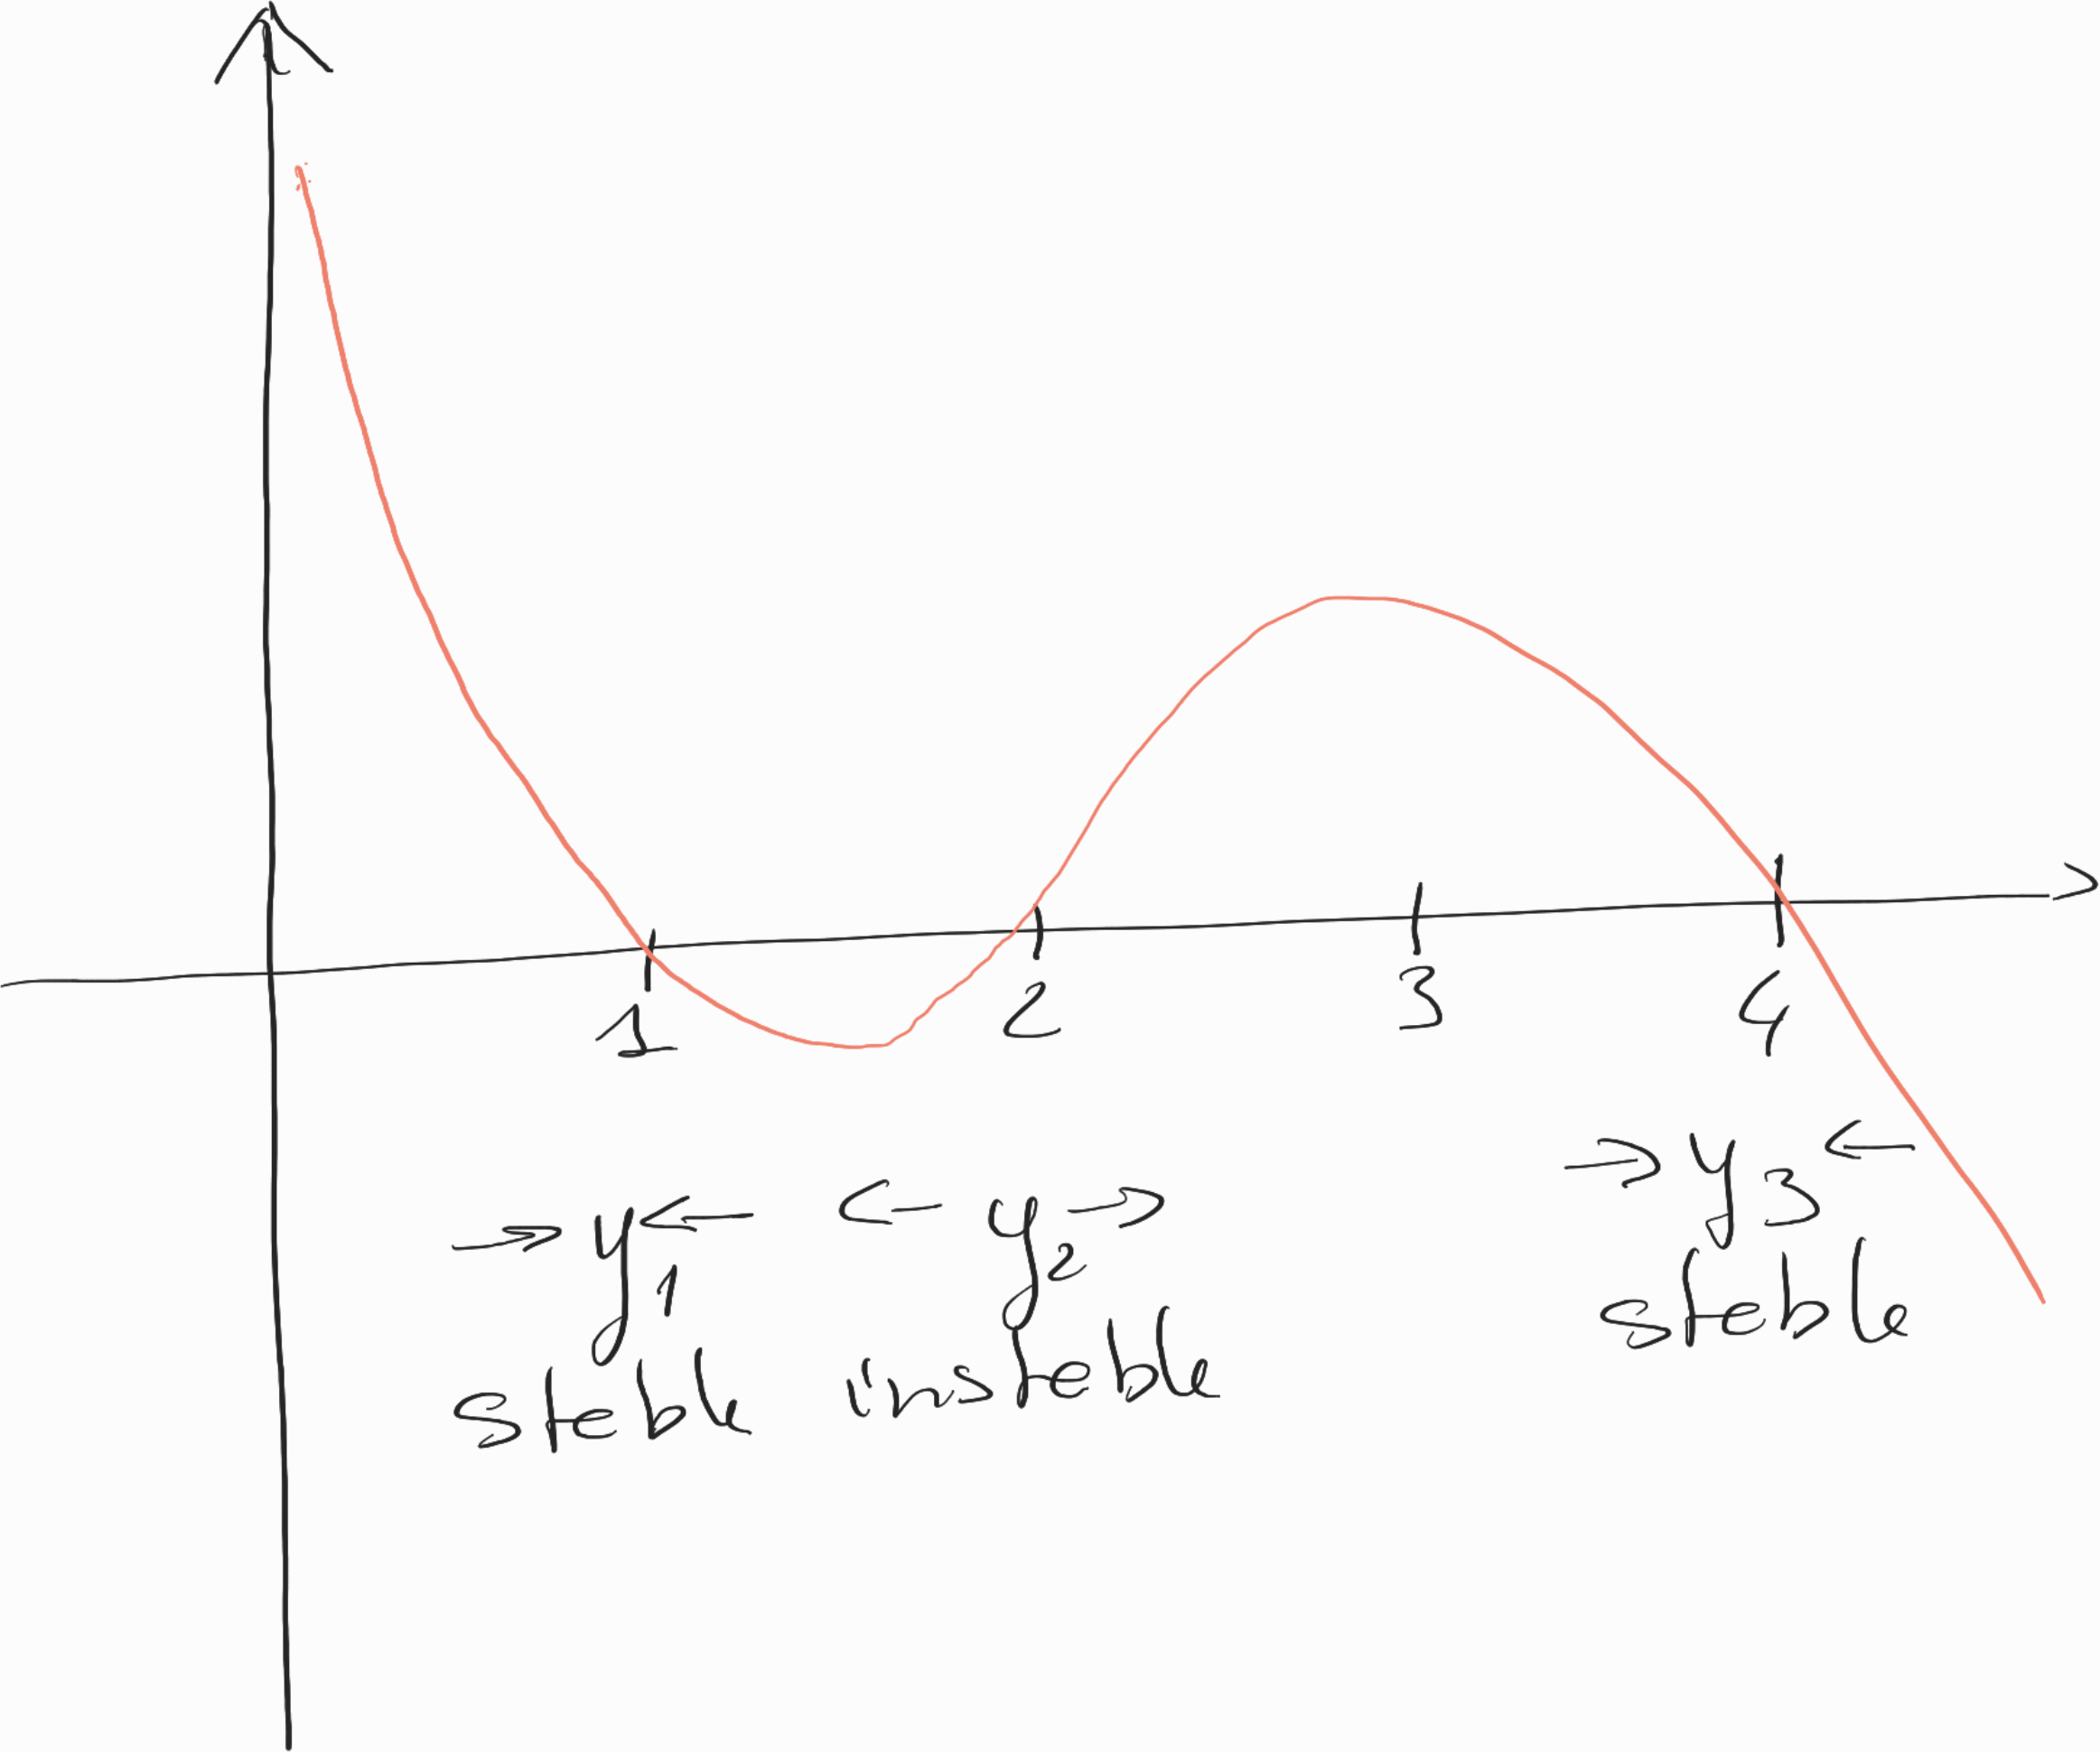
\includegraphics[width=.5\textwidth]{TD-SUbioL3-TD2Exo2}
  $$
}




%-------------------------------------------------------------------------------
\subsubsection{Système dynamique en $y^5$ \todo{}}
%-------------------------------------------------------------------------------

On souhaite déterminer les points d'équilibre (et leur nature) du système
$$
\dot y = F(y) = \mu y + 2 y^3 - y^5.
$$
On a 
$$
F(y) = y(\mu + y^2 - y^4)
$$
qui s'annule pour $y = 0$ et pour les solutions de $(\mu + 2 y^2 - y^4)$. En posant, $z = y^2$, $\mu + 2 z - z^2 = 0$ admet des solutions si $\Delta =  4(1 + \mu) \geq 0$, soit $\mu \geq -1$. Ces solutions sont alors $z^* = -1 \pm \sqrt{1+\mu}$. La seule solution possiblement positive est $z^* = -1 + \sqrt{1+\mu}$ et elle l'est ssi $\mu > 1$. \\
Le système admet donc un unique point fixe $x^*=0$ si $\mu < 1$ et un second point fixe $x^* = -1+\sqrt{1+\mu}$ si $\mu > 1$. \\
On a de plus
$$
F'(x) = \mu + 3 y^2 - 5y^4
$$
dont le signe est celui de $\mu$ pour $x=0$ et \todo{nature de $x^* = -1+\sqrt{1+\mu}$ si $\mu > 1$.}


%-------------------------------------------------------------------------------
\subsubsection{Modèle de Allee \todo{}}
%-------------------------------------------------------------------------------

% Voir \url{https://umr5558-shiny.univ-lyon1.fr/web/}

On considère une version canonique du modèle de dynamique de population proposé par W.C. Allee en 1949. En notant $x(t)$ la taille d'une population au temps $t$, ce modèle pose que 
\begin{equation} \label{eq:modAllee}
  \dot x = f(x) = x (x-1) (2-x).
\end{equation}

\bigskip 
\paragraph{\'Etude des points stationnaires}
\begin{enumerate}
  \item Déterminer les trois points stationnaires $x_1^* < x_2^* < x_3^*$ du système et étudier leur stabilité.
  \solution{
    $f(x)$ s'annule pour $x_1^* = 0$, $x_2^* =1$ et $x_3^* = 2$. \\
    Concernant leur stabilité, puisque $f(x) = -x^3 + 3x^2 - 2x$, on a $f'(x) = -3x^2 + 6x - 2$ et donc
    \begin{align*}
      f'(x_1^* = 0) & = -2 < 0 : & & \text{$x_1^*$ est un équilibre stable;} \\
      f'(x_2^* = 1) & = + 1 > 0 : & & \text{$x_2^*$ est un équilibre instable;} \\
      f'(x_3^* = 2) & = -8 < 0  :& & \text{$x_3^*$ est un équilibre stable.}
    \end{align*}
  }
  \item Tracer le diagramme de stabilité et donner l'allure des solutions du système \eqref{eq:modAllee}.
  \solution{
  Le diagramme de stabilité est donc le suivant
  $$
  \begin{tikzpicture}
    \node[] (x0) at (-1*\edgeunit, 0) {}; 
    \node[] (x01) at (-0.5*\edgeunit, 0) {}; 
    \node[] (x1) at (0*\edgeunit, 0) {$x_1^*$}; 
    \node[] (x12) at (0.5*\edgeunit, 0) {}; 
    \node[] (x2) at (1*\edgeunit, 0) {$x_2^*$}; 
    \node[] (x23) at (1.5*\edgeunit, 0) {}; 
    \node[] (x3) at (2*\edgeunit, 0) {$x_3^*$}; 
    \node[] (x34) at (2.5*\edgeunit, 0) {}; 
    \node[] (x4) at (3*\edgeunit, 0) {}; 
    
%     \draw[-] (x0) -- (x4);
    \draw[->] (x01) -- (x1); \draw[->] (x12) -- (x1);  
    \draw[->] (x2) -- (x12); \draw[->] (x2) -- (x23); 
    \draw[->] (x23) -- (x3); \draw[->] (x34) -- (x3);  
  \end{tikzpicture}
  $$
  et les solutions ont les allures suivantes :
  $$
  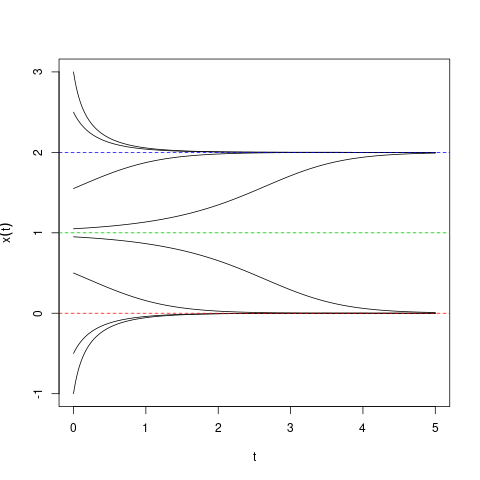
\includegraphics[width=0.5\textwidth, trim=0 10 20 50, clip=]{Allee-solutions}
  $$
  }
  \item Interpréter ces résultats et notamment le statut de l'équilibre $x_2^*$.
  \solution{
    Les solutions $x_1^*$ et $x_3^*$ ont pour bassins d'attraction respectifs $(-\infty, x_2^*[$ et $]x_2^*, \infty)$. L'équilibre $x_2^*$ constitue une valeur seuil : si $x(0) > x_2^*$, la taille de la population tend vers $x_ 3^* > 0$, alors que si $x(0) < x_2^*$, la taille de la population tend vers $x_1^* = 0$, c'est-à-dire vers l'extinction. 
  }
\end{enumerate}

\bigskip 
\paragraph{Solution.}
\begin{enumerate}
  \item Montrer que la fonction
  $$
  u(t) = 1 + \frac1{\sqrt{1 + 3 e^{-2t}}}
  $$
  est solution du système \eqref{eq:modAllee}. \\
  ({\sl On pourra commencer par étudier la fonction $v(t) = 1 + 3 e^{-2t}$.})
  \solution{
    Comme suggéré par l'énoncé, on calcule $\dot v(t) = -6 e^{-2t}$ et on remarque que $\dot v = 2 (1 - v)$. On remarque ensuite que, puisque $u(t) = 1 + 1/\sqrt{v(t)}$, on a
    $$
    \dot u 
    = -\frac{\dot v}{2 v^{3/2}}
    = \frac{v - 1}{v^{3/2}}.
    $$
    On remarque d'autre part que
    $$
    f(u) 
    = \left(1 + \frac1{\sqrt{v}}\right) \left(\frac1{\sqrt{v}}\right) \left(1 - \frac1{\sqrt{v}}\right)
    = \frac1{\sqrt{v}} \left(1 - \frac1u\right)
    = \frac{v-1}{v^{3/2}}.
    $$
    On a donc $\dot u = f(u)$ : la fonction $u$ proposée est bien solution du système \eqref{eq:modAllee}.
  }
  \item Déterminer $u(0)$ et en déduire la limite vers laquelle tend la taille de la population.
  \solution{
    On a $u(0) = 1 + 1/\sqrt{4} = 3/2$ qui se situe dans le bassin d'attraction de $x_3^*$ : la taille de la population tend donc vers $x_3^* = 2$. \\
    {\sl Alternativement}, on peut calculer directement $\lim_{t \to \infty} u(t) = 2$.
  }
\end{enumerate}


%-------------------------------------------------------------------------------
\subsection{Systèmes dynamiques en dimension 2}
%-------------------------------------------------------------------------------

\bigskip
\todo{Examen L3-Bio-SU 2022-23 : Exercice 2} 

%-------------------------------------------------------------------------------
\subsubsection{Système dynamique linéaire.} 
%-------------------------------------------------------------------------------

On considère le système dynamique suivant
$$
\left\{\begin{array}{rcl}
        \dot x & = & -a_1 x + b_1 y + c_1 \\ 
        \dot y & = & -a_2 x + b_2 y + c_2
        \end{array}\right.
$$
où tous les coefficients constants sont strictement positifs.
\begin{enumerate}
  \item À quelle condition y a-t-il un unique équilibre ? Lorsque c’est le cas, à quelle condition est-il stable ?
  \solution{\todo{}}
  \item Lorsqu’il n’existe pas d’équilibre unique, représenter les deux isoclines (c'est à dire les ensemble de points ou s'annule $\dot x$ d'une part et $\dot y$ d'autre part). Y a-t-il une infinité d’équilibres ou aucun équilibre ?
  \solution{\todo{}}
  \item Représenter les orbites dans le plan de phase.
  \solution{\todo{}}
\end{enumerate}


%-------------------------------------------------------------------------------
\subsubsection{Système dynamique quadratique} \label{SystDyn-Quadratique}
%-------------------------------------------------------------------------------

On considère le système dynamique d’activation réciproque avec compétition intraspécifique suivant 
$$
%   \SR{
%   \left\{\begin{array}{rcl}
%          \dot x & = & r y - cx^2 \\ 
%          \dot y & = & r x - cy^2 
%          \end{array}\right.
%   }{
\left\{\begin{array}{rcl}
        \dot x & = & a y - x^2 \\ 
        \dot y & = & a x - y^2 
        \end{array}\right.
%   }
$$
%   où $r$ et $c$ sont deux constantes strictement positives.
où $a$ est une constante strictement positive.
\begin{enumerate}
  \item Déterminer les équilibres de ce modèle.
  \solution{$(x=0, y=0)$ est un point d'équilibre trivial. L'autre point d'équilibre s'obtient en résolvant
  $$
  \left\{\begin{array}{rcl}
          a y & = & x^2 \\
          a x & = & y^2
        \end{array}\right.
  \quad \Leftrightarrow \quad
  \left\{\begin{array}{rcl}
          y & = & x^2 / a \\
          a x & = & x^4 / a^2
        \end{array}\right.
  \quad \Leftrightarrow \quad
  \left\{\begin{array}{rcl}
          y & = & x^2 / a \\
          a^3 & = & x^3
        \end{array}\right.
  \quad \Leftrightarrow \quad
  x^* = y^* = a.
  $$}
  \item Donner la nature de chacun de ces deux équilibres.
  \solution{En notant
  $$
  F(x, y) = \left[\begin{array}{rcl} 
                    F_1(x, y) & = & ay - x^2 \\
                    F_2(x, y) & = & ax - y^2
                  \end{array}\right],
  $$
  on a
  $$
  J_{(x, y)} F = \left[\begin{array}{cc}-2x & a \\ a & -2y\end{array}\right].
  $$
  \begin{description}
    \item[Point $(0, 0)$:] on a
    $$
    J_{(0, 0)} F = \left[\begin{array}{cc}0 & a \\ a & 0\end{array}\right]
    \quad \Rightarrow \quad
    P(\lambda) = \lambda^2 - a^2
    $$
    qui s'annule pour $\lambda = \pm a$. Des vecteurs associés à $a$ et $-a$ sont, respectivement $[1 \; 1]^\top$ et $[-1 \; 1]^\top$. \\
    $(0, 0)$ est un équilibre instable dans la direction de la première bissectrice et stable dans celle de la seconde.
    \item[Point $(a, a)$:] on a
    $$
    J_{(0, 0)} F = \left[\begin{array}{cc}-2a & a \\ a & -2a\end{array}\right]
    \quad \Rightarrow \quad
    P(\lambda) = \lambda^2 - a^2
    \quad \Rightarrow \quad
    P(\lambda) = \lambda^2 - 4 a \lambda + 3 a^2
    $$
    qui s'annule pour $\lambda = -a$ et $\lambda = -3a $. \\
    $(a, a)$ est donc un équilibre stable.
  \end{description}
  }
  \item Que se passe-t-il si $x(0) = y(0) > 0$ ? Représenter l’allure des trajectoires dans le plan de phase. 
  \solution{
  On peut remarquer que 
  $$
  \dot x \geq 0 \quad \Leftrightarrow \quad y \geq x^2/a, \qquad \qquad
  \dot y \geq 0 \quad \Leftrightarrow \quad y \leq \sqrt{a x}.
  $$
  $$
  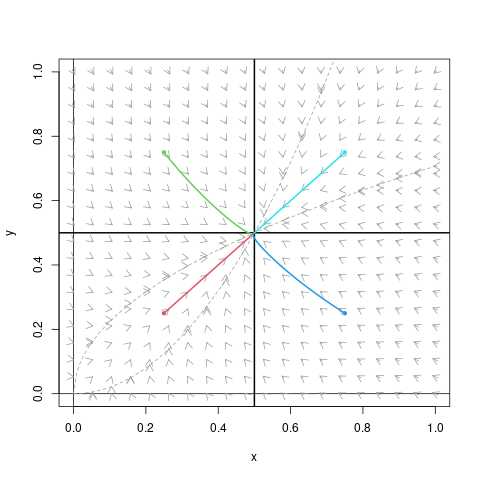
\includegraphics[width=.45\textwidth, trim=0 10 20 20, clip=]{ActivationReciproque}
  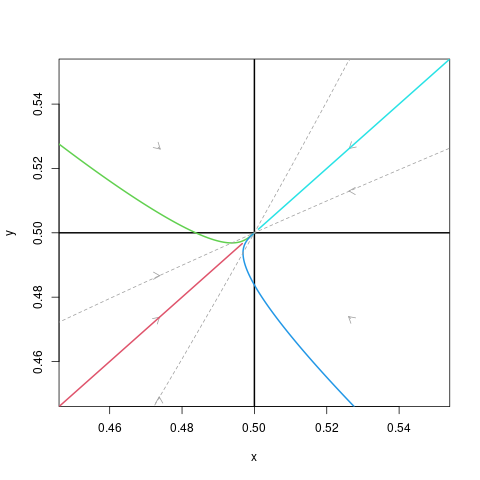
\includegraphics[width=.45\textwidth, trim=0 10 20 20, clip=]{ActivationReciproque-zoom}
  $$
  Toutes les trajectoires convergent vers $(a, a)$.
  \begin{description}
    \item[$(x_0 < a, y_0 < a)$:] la trajectoire converge directement vers $(a, a)$.
    \item[$(x_0 < a, y_0 > a)$:] la trajectoire franchit l'axe $y = a$ avant de revenir en $(a, a)$.
    \item[$(x_0 > a, y_0 > a)$:] la trajectoire converge directement vers $(a, a)$.
    \item[$(x_0 > a, y_0 < a)$:] la trajectoire franchit l'axe $x = a$ avant de revenir en $(a, a)$.
  \end{description}
  }
\end{enumerate}



%-------------------------------------------------------------------------------
\subsubsection{Système proie prédateur} 
%-------------------------------------------------------------------------------

On considère le système proie-prédateur suivant
\begin{equation} \label{eq:L3bioProiePredateur}
\left\{\begin{array}{rcl}
        \dot x & = & \displaystyle{x \left(1 - \frac{x}2\right) - \frac{xy}{1+x}} \\
        \dot y & = & \displaystyle{\frac{x-1}{x+1} y}
       \end{array}\right..
\end{equation}
% dans laquelle $x$ désigne la concentration d'un métabolite : \eqref{eq:L3BioSUTD2E2} modélisant l'ensemble des réactions biochimiques impliquées dans la production/dégradation de ce métabolite.

\begin{enumerate}
\item Qui sont les proies, qui sont les prédateurs ?
  \solution{$x =$ proies, $y = $ prédateurs : 
    \begin{itemize}
    \item Le terme d'interaction $xy$ intervient avec un signe négatif dans le taux de croissance $\dot x$, ce qui est caratéristique du comportement d'une population de proies confrontées à des prédateurs.
    \item Pour $x=0$, on obtient $\dot y = -y$ qui décrit un comportement d'une population de prédateurs qui s'éteint en l'absence de proie. 
    \end{itemize}}
\item Déterminer les points stationnaires du systèmes.
  \solution{En distinguant les cas $y = 0$ et $y \neq 0$, on vérifie facilement que
  $$
  m^*_1 = \left(\begin{array}{c}0 \\ 0\end{array}\right), \qquad
  m^*_2 = \left(\begin{array}{c}2 \\ 0\end{array}\right), \qquad
  m^*_3 = \left(\begin{array}{c}1 \\ 1\end{array}\right)
  $$
  sont les seuls points stationnaires.}
\item Montrer que $y=0$ est une solution du système. Quel est le comportement de $x$ dans ce cas ?
  \solution{$y \equiv 0$ satisfait la seconde équation du système. La première équation devient alors $\dot x = x \left(1 - x/2\right)$ : la population des proies évolue selon un modèle logistique.}
\item Déterminer la matrice jacobienne $J_{x, y}$ du système
  \solution{On a
  $$
  J_{x, y} = \left[\begin{array}{ccc}
                   \displaystyle{(1 - x) - \frac{y}{(1+x)^2}} & & 
                   \displaystyle{\frac{-x}{1+x}} \\
                   \displaystyle{\frac{2 y}{(x+1)^2}} & & 
                   \displaystyle{\frac{x-1}{x+1}}
                  \end{array}\right]
  $$}
  \item \'Etudier la stabilité des points stationnaires.
  \solution{
  \begin{description}
  \item[$m^*_1 = (0, 0) : $] on a 
    $$
    J_{m^*_1} = \left[\begin{array}{ccc}
                    {1} & & 
                    {0} \\
                    {0} & & 
                    {-1/2}
                    \end{array}\right]
    $$
    dont les valeurs propres sont 1 (associée à $u = (1, 0)$) et $-1/2$ (associée à $u = (0, 1)$). \\
    Il s'agit donc d'un point selle : l'équilibre est instable. Plus précisément, il est instable dans la direction de l'axe des $x$ (en l'absence de prédateur, la population de proies croît) et stable dans la direction de l'axe des $y$ (en l'absence de proie, les prédateurs s'éteignent).
  \item[$m^*_2 = (0, 0) : $] on a 
    $$
    J_{m^*_2} = \left[\begin{array}{ccc}
                    {-1} & & 
                    {-2/3} \\
                    {0} & & 
                    {1/3}
                    \end{array}\right]
    $$
    qui est triangulaire : ses valeurs propres sont $-1$ (associée à $u = (1, 0)$) et $1/3$ (associée à $u = (0, 1)$). \\
    Il s'agit aussi d'un point selle : l'équilibre est donc instable. Plus précisément, il est stable dans la direction de l'axe des $x$ (en l'absence de prédateur, la population de proies tend vers 2) et instable dans la direction de l'axe des $y$ (pour $x=2$, la population des prédateurs croît).
  \item[$m^*_3 = (1, 1) : $] on a 
    $$
    J_{m^*_3} = \left[\begin{array}{ccc}
                    {-1/4} & & 
                    {-1/2} \\
                    {1/2} & & 
                    {0}
                    \end{array}\right]
    $$
    dont le polynôme caractéristique est $P(\lambda) = \lambda^2 + \lambda/4 + 1/4.
    $. Son discriminant est $\Delta = 1/16 - 1 = -15/16$ : les valeurs propres sont donc $\lambda_1 = (-1 + i\sqrt{15})/8$ et $\lambda_2 = (-1 -\sqrt{15})/8$. \\
    Les parties réelles des valeurs propres sont négatives, donc l'équilibre est stable.
  \end{description}}
  \item Tracer le comportement du système aux abords de chacun des points stationnaires.
  \solution{Quelques exemples de trajectoires
  $$
  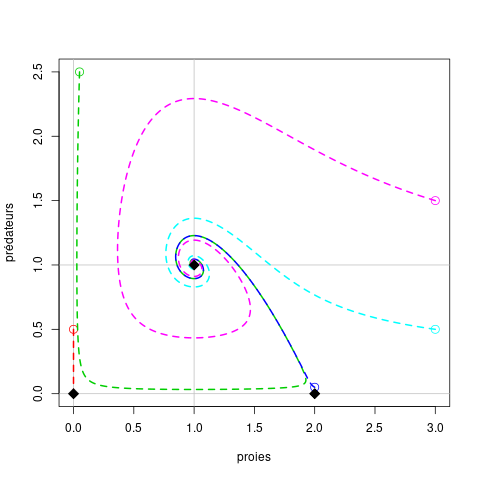
\includegraphics[width=.5\textwidth, trim=0 0 30 60, clip=]{L3bioSU-ProiePredateur-paths}
  $$
  $$
  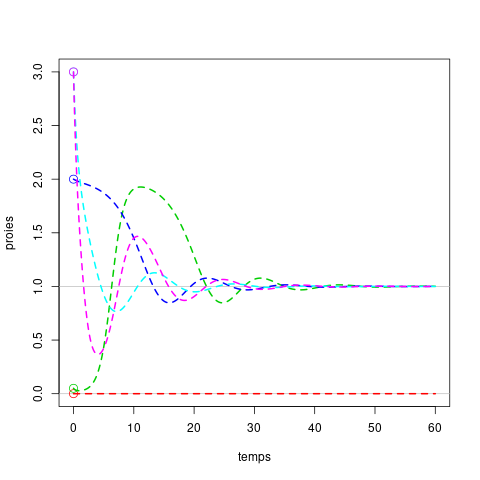
\includegraphics[width=.45\textwidth, trim=0 0 30 60, clip=]{L3bioSU-ProiePredateur-proies}
  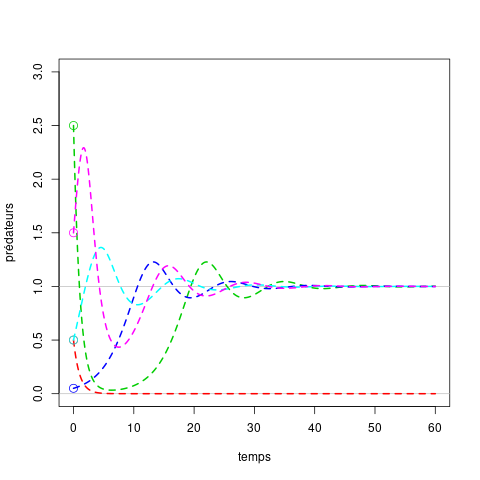
\includegraphics[width=.45\textwidth, trim=0 0 30 60, clip=]{L3bioSU-ProiePredateur-predateurs}
  $$
  }
\end{enumerate}


\bigskip
Cycle limite \todo{Voir exemple 1, p 195, Perko, 2001} 

%-------------------------------------------------------------------------------
\subsubsection{Modèle de Lotka-Volterra avec densité dépendance} 
%-------------------------------------------------------------------------------

\paragraph{Rappel.}
En notant 
\begin{itemize}
  \item $x(t)$ une variable proportionnelle au nombre de proies et
  \item $y(t)$ une variable proportionnelle au nombre de prédateurs,
\end{itemize}
le modèle Lotka-Volterra classique s'écrit, 
\begin{equation} \label{eq:LV}
\left\{\begin{array}{rcr}
        \dot x & = & r x (1 - y), \\ 
        \dot y & = & - m y (1 - x).
        \end{array}\right.
\end{equation}
Notamment, ce modèle admet deux points d'équilibre en $(x=0, y=0)$ et $(x=1, y=1)$.

\paragraph{Prise en compte d'une densité-dépendance.}
On considère ici un modèle de Lotka-Volterra avec densité dépendance. Plus précisément, en supposant le taux de croissance des proies égale à 1 ($r = 1$), on pose le modèle
\begin{equation} \label{eq:LVDD}
\left\{\begin{array}{rcr}
        \dot x & = & x (1 - y - ax), \\ 
        \dot y & = & - m y (1 - x), 
        \end{array}\right.
\end{equation}
où les paramètres $m$ et $a$ sont strictement positifs. 
% On remarque que le cas $a=0$ correspond au modèle de Lotka-Volterra classique (avec $r=1$).

\bigskip
\paragraph{Interprétation du modèle \eqref{eq:LVDD}.}
\begin{enumerate}
  \item Interpréter les paramètres $m$ et $a$ du modèle \eqref{eq:LVDD}.
  \solution{$m$ est le taux de mort des prédateurs en absence de proies (si $x(0)= 0$, $y(t) = y_0 e^{-mt}$). $a$ rend compte de la compétition entre les proies, c'est-à-dire de la limitation des ressources du milieu.}
  \item Déterminer les points d'équilibre du système \eqref{eq:LVDD}.
  \solution{
  L'isocline $\{\dot x = 0\}$ est $\Ical_x = \{x = 0\} \cup \{y = 1 - ax\}$ et l'isocline $\{\dot y = 0\}$ est $\Ical_y = \{y = 0\} \cup \{x = 1\}$. Les points d'équilibre sont donc $(0, 0)$, $(0, 1/a)$ et $(1, 1-a)$.}
  \item Expliquer la position du point d'équilibre $(x^*, y^*)$ non nul (c'est-à-dire pour lequel $x^*$ et $y^*$ sont non nuls) par rapport au point d'équilibre non nul du modèle de Lotka-Volterra classique \eqref{eq:LV}.
  \solution{L'équilibre non-trivial du modèle de Lotka-Volterra est le point $(1, 1)$. Le point d'équilibre des proies est conservé ($x^* = 1$), mais celui des prédateurs diminue $y^* = 1-a < 1$ : la contrainte imposée par le milieu au proies nuit, {\it in fine} à la population des prédateurs.}
\end{enumerate}

\bigskip
\paragraph{Questions intermédiaires (I).}
Soit la fonction $f: \Rbb^{*+} \mapsto \Rbb$, définie par $f(x) = \sqrt{x(x+1)} - x$.
\begin{enumerate}
  \setcounter{enumi}{3}
  \item Montrer que $f(x) > 0$. \label{q:LVDD-f1}
  \solution{On a $\sqrt{x(x+1)} > \sqrt{x^2} = x$, donc $f(x) > 0$.
  }
  \item Montrer que $f(x) < 1/2$. \label{q:LVDD-f2}
  \solution{On a
  $$
  f(x) < \frac12 
  \qquad \Leftrightarrow \qquad
  x(x+1) < \left(x + \frac12\right)^2
  \qquad \Leftrightarrow \qquad
  x^2 + x < x^2 + x + \frac14
  $$
  qui est toujours vrai.
  }
\end{enumerate}

\bigskip 
\paragraph{Questions intermédiaires (II).}
Soit la matrice $J^*$ définie par
\begin{equation} \label{eq:LVDD-Jstar}
  J^* = \left(\begin{array}{cc}
              -a & -1 \\ m(1-a) & 0
              \end{array}\right).
\end{equation}

\bigskip
\begin{enumerate}
  \setcounter{enumi}{5}
  \item Déterminer le polynôme caractéristique $P$ de $J^*$.
  \solution{$P(\lambda) = \lambda^2 + a \lambda + m(1-a)$.}
  %
  \item Montrer que les valeurs propres de $J^*$ sont réelles si et seulement si $a \geq a_1 = 2 f(m)$, où $f$ est la fonction définie en (I). 
  ({\sl On pourra étudier le discriminant $\Delta$ de $P$ comme une fonction de $a$.})
  \solution{La nature des valeurs propres de $J^*$ est donnée par le signe du discriminant de $P$ : $\Delta = \Delta(a) = a^2 + 4am - 4m$ qui est lui même un polynôme en $a$. \\
  Son discriminant est $\delta = 16m^2 + 16m = 16 m(m+1)$ est positif puisque $m$ est positif. 
  $\Delta(a)$ admet donc deux racines réelles:  $-2 (m + \sqrt{m(m+1)})$, qui est négative, et $a_1 = 2 (\sqrt{m(m+1)} - m) = 2f(m)$ qui est strictement positive d'après la question \ref{q:LVDD-f1}. 
  \\ $\Delta(a)$ est donc positif dès que $a \geq a_1 = 2 f(m)$ et $P$ admet alors deux racines réelles (égales si $a = a_1$). 
  }
  %
  \item Montrer que $a_1 < 1$ et que si $a > 1$, les valeurs propres de $J^*$ sont de signes différents. \label{q:racinePstar}
  \solution{
  La question \ref{q:LVDD-f2} nous assure que $a_1 = 2 f(m) < 1$, puisque $f(x) < 1/2$ pour tout $x \geq 0$. \\
  Si $a > a_1$, $P$ admet pour racines réelles $\lambda_1 = -(a +\sqrt{\Delta(a)})/2$, qui est toujours négative, et $\lambda_2 = (-a + \sqrt{\Delta(a)})/2$, qui est est positive dès que 
  $$
  \sqrt{\Delta(a)} \geq a
  \qquad \Leftrightarrow \qquad
  a^2 + 4am - 4m \geq a^2
  \qquad \Leftrightarrow \qquad
  a \geq 1.
  $$
  $J^*$ a donc des valeurs propres de racines distinctes dès que $a > 1 > a_1$. \\ 
  Alternativement, par les propriétés du polynôme caractéristique d'une matrice de $\Mcal_2$, $\lambda_1$ et $\lambda_2$ sont de même signe ssi $\lambda_1 \lambda_2 = |J^*| = m(1-a) > 0$, c'est-à-dire si $a <1$, puisque $m > 0$.
  }
\end{enumerate}
  

\bigskip
\paragraph{Stabilité du point d'équilibre non nul.}
On s'intéresse maintenant à la stabilité du point d'équilibre $(x^*, y^*)$ non nul. 
\begin{enumerate}
  \setcounter{enumi}{8}
  \item Déterminer la matrice jacobienne du système en un point $(x, y)$ quelconque.
  \solution{
  $$
  J = \left(\begin{array}{cc}
            -2ax + (1-y) & -x \\ my & m(x-1) 
            \end{array}\right).
  $$
  }
  \item En déduire que la matrice jacobienne en $(x^*, y^*)$ est égale à la matrice $J^*$ définie à l'équation \eqref{eq:LVDD-Jstar}.
  \solution{Direct.}
  \item \'Etudier la nature de l'équilibre $(x^*, y^*)$ en fonction de la position de $a$ par rapport aux deux valeurs seuils $a_1$ et $1$ : $a < a_1$, $a_1 < a < 1$ ou $a > 1$.
  ({\sl On ne s'attardera pas sur les cas limites $a = a_1$ et $a = 1$}.)
  \solution{
  \begin{description}
    \item[$a < a_1$ :] dans ce cas, $\Delta(a) < 0$ et les valeurs propres de $J*$ sont $\lambda_1$ et $\lambda_2$ calculées à la question \ref{q:racinePstar}, qui sont complexes mais dont les parties réelles sont négatives puisque $a > 0$. L'équilibre $(x^*, y^*)$ est donc un équilibre stable.
    \item[$a_1 < a < 1$ :] dans ce cas, $\Delta(a) > 0$ et les valeurs propres $\lambda_1$ et $\lambda_2$ sont toutes les deux réelles et négatives : l'équilibre $(x^*, y^*)$ est donc toujours stable.
    \item[$a > 1$ :] $\lambda_1$ est toujours négative mais $\lambda_2$ devient positive et $(x^*, y^*)$ devient alors instable.
  \end{description}
  Les figures suivantes donnent respectivement les parties réelles $Re(\lambda)$ et imaginaires $Im(\lambda)$  des valeurs propres $\lambda_1$ et $\lambda_2$ en fonction de $a$ pour $m=1/2$. 
  $$
  \begin{array}{c}
    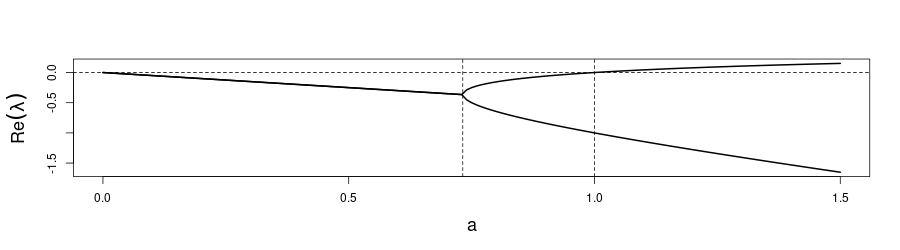
\includegraphics[width=.8\textwidth, trim=0 0 0 50, clip=]{LotkaVolterraDD-m0.5-eigenValueReal.png} \\
    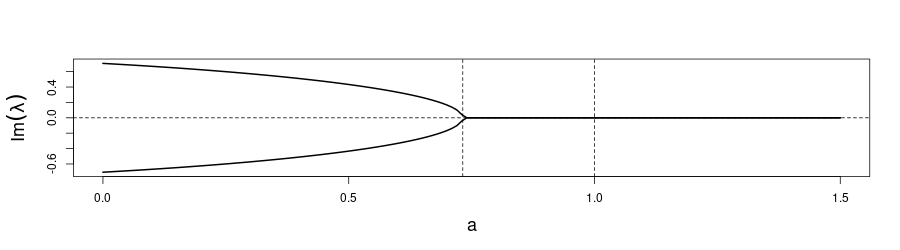
\includegraphics[width=.8\textwidth, trim=0 0 0 50, clip=]{LotkaVolterraDD-m0.5-eigenValueImaginary.png} 
  \end{array}
  $$
  La bifurcation se produit en $a = a_1$ et l'une des valeurs propres devient positive pour $a = 1$.
  }
\end{enumerate}

\bigskip
\paragraph{Trajectoires.}
Les trajectoires ($i$), ($ii$) et ($iii$) suivantes ont été obtenues par intégration numérique avec $m = 1/2$ et partant de l'état initial $(x_0 = 2,\;  y_0 = 3/2)$ pour trois valeurs de $a$ différentes :
$$
\begin{array}{ccc}
  (i) & (ii) & (iii) \\
  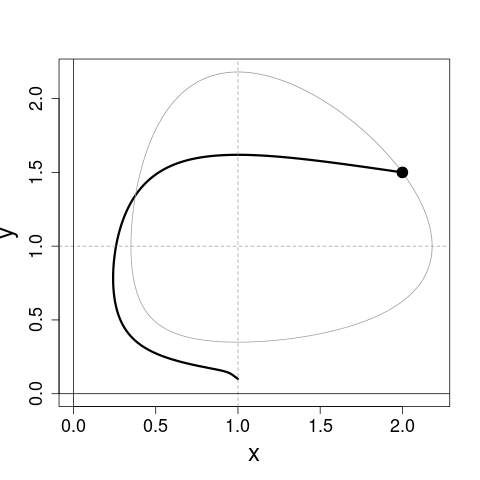
\includegraphics[width=.32\textwidth, trim=0 0 0 50, clip=]{LotkaVolterraDD-m0.5-a0.9.png} &
  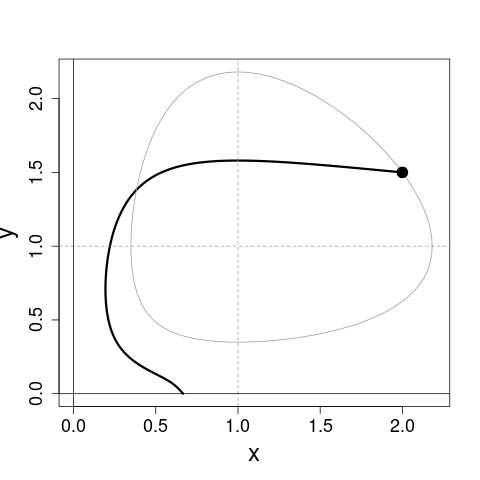
\includegraphics[width=.32\textwidth, trim=0 0 0 50, clip=]{LotkaVolterraDD-m0.5-a1.5.png} &
  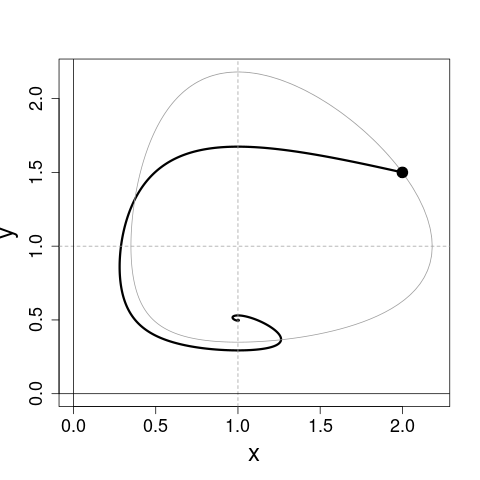
\includegraphics[width=.32\textwidth, trim=0 0 0 50, clip=]{LotkaVolterraDD-m0.5-a0.5.png}
\end{array}
$$
La courbe grise indique la trajectoire du modèle de Lotka-Volterra \eqref{eq:LV} sans densité-dépendance ($m = 1/2$, $a = 0$), partant du même point initial. Les repères grisés indiquent le point d'équilibre de ce même modèle \eqref{eq:LV}.

\begin{enumerate}
  \setcounter{enumi}{11}
  \item Associer chacune des trajectoires ($i$), ($ii$) et ($iii$) à l'une des trois valeurs de $a$ : $a = 1/2$, $a = 9/10$ et $a = 3/2$.
  \solution{On a dans ce cas $a_1 = 2 f(1/2) = \sqrt{3} - 1 \simeq 0.73$.
  \begin{description}
    \item[$a = 1/2 < a_1$ :] le système possède un équilibre stable en ($x^* = 1, y^* = 1/2$) et les valeurs propres de $J^*$ possèdent une partie imaginaire non nulle qui induit un enroulement autour de l'équilibre : on reconnaît la trajectoire ($iii$).
    \item[$a_1 < a = 9/10 < 1$ :] le système possède un équilibre stable en ($x^* = 1, y^* = 1/10$) mais les valeurs propres de $J^*$ sont réelles et négatives : le système tend vers l'équilibre sans enroulement : on reconnaît la trajectoire ($i$).
    \item[$a = 3/2 > a_1$ :] le système possède un équilibre instable en ($x^* = 1, y^* = -1/2$) que le système n'atteint jamais, du fait de l'extinction des prédateurs ($y(t) \to 0$) : on reconnaît la trajectoire ($ii$).
  \end{description}
  }
  \item Donner la limite de $x(t)$ quand $t$ tend vers l'infini dans le cas ($ii$).
  \solution{
  Dans ce cas, $y(t)$ tend vers 0 quand $t \to\infty$, le système \eqref{eq:LVDD-Jstar} devient donc simplement $\dot x = F(x)$ avec $F(x) = x (1 - ax)$. Ce système admet deux points d'équilibre en $x_1 = 0$ et $x_2 = 1/a$ et seul le second est stable (car $F'(x_1) > 0$ et $F'(x_2) < 0$). \\
  Après extinction des prédateurs, la population des proies tend donc vers un des équilibres 'nuls' : $(x_2 = 1/a = 2/3, y=0)$. Du fait de la densité-dépendance, la population des proies n'explose donc pas, contrairement au modèle de Lotka-Volterra classique.
  }
\end{enumerate}


%-------------------------------------------------------------------------------
\subsubsection{Système de Lorenz en 2 dimensions} 
%-------------------------------------------------------------------------------

On considère une version réduite à deux dimensions du système de Lorenz, c'est-à-dire à un couple $(x(t), y(t))_{t \geq 0}$ satisfaisant les conditions initiales
$$
x(0) = x_0, \qquad y(0) = y_0
$$
et vérifiant le système d'équations différentielles ordinaires
\begin{equation*} % \label{eq:lorenz2D}
  \left\{\begin{array}{rcl}
    \dot x & = a x - xy \\
    \dot y & = x^2 - by
  \end{array}\right.
\end{equation*}
où les coefficients $a$ et $b$ sont strictement positifs.

\paragraph{Détermination des points stationnaires et de leur stabilité.}
\begin{enumerate}
  \item Montrer que le système admet trois points stationnaires.
  \solution{
    En annulant simultanément
    $$
    F_1(x, y) = a x - xy, \qquad F_2(x, y) = x^2 - by,
    $$
    on détermine que le vecteur gradient est nul aux points 
    $$
    O = (0, 0), \qquad A = (\sqrt{ab}, a) \quad \text{et} \quad B = (-\sqrt{ab}, a).
    $$
  }
  \item Déterminer la matrice Jacobienne du système.
  \solution{
  On a
  $$
  J f = \left[\begin{array}{cc} a-y & -x \\ 2x & -b \end{array} \right].
  $$
  }
  \item En déduire la nature (stable ou instable) de chacun des points stationnaires.
  \solution{
  \begin{description}
    \item[$O = (0, 0)$ :] On a
    $$
    J_0 f = \left[\begin{array}{cc} a & 0 \\ 0 & -b \end{array} \right],
    $$
    dont les valeurs propres ($\lambda_1 = a, \lambda_2 = b)$ sont de signes opposés : $O$ est donc instable. Plus précisément, il est instable le long de l'axe des $x$ et stable le long de l'axe des $y$.
    \item[$A = (\sqrt{ab}, a)$ :] On a
    $$
    J_A f = \left[\begin{array}{cc} 0 & -\sqrt{ab} \\ 2\sqrt{ab} & -b \end{array} \right],
    $$
    donc $\tr(J_A f) = -b < 0$ et $\det(J_A f) = 2ab > 0$. Les deux valeurs propres sont donc de même signe et négatives : $A$ est donc un équilibre stable. \\
    {\sl Alternative :} Le polynôme caractéristique
    $$
    P_A(\lambda) = \lambda^2 + b \lambda + 2 ab
    $$
    a pour discriminant $\Delta = b^2 - 8 ab$. 
    \begin{itemize}
      \item Si $0 < a < b/8$, $\Delta$ est positif et les valeurs propres sont 
      $$
      \lambda_1 = \frac12 \left(-b + \sqrt{\Delta}\right) 
      \quad \text{et} \quad
      \lambda_2 = \frac12 \left(-b - \sqrt{\Delta}\right).
      $$
      comme de plus $\Delta < b^2$, les deux valeurs propres sont négatives, donc $A$ est stable.
      \item Si $a > b/8$, $\Delta$ est négatif et les valeurs propres sont 
      $$
      \lambda_1 = \frac12 \left(-b + i \sqrt{|\Delta|}\right) 
      \quad \text{et} \quad
      \lambda_2 = \frac12 \left(-b - i \sqrt{|\Delta|}\right),
      $$      
      dont la partie entière commune est $-b < 0$, donc $A$  est également stable.
    \end{itemize}
    \item[$B = (-\sqrt{ab}, a)$ :] On a alors    
    $$
    J_B f = \left[\begin{array}{cc} 0 & \sqrt{ab} \\ -2\sqrt{ab} & -b \end{array} \right]
    $$
    qui a la même trace et le même déterminant que $J_A f$ : $B$ est donc également stable. \\
    {\sl Alternative :} Le polynôme caractéristique de $J_B f$ est le même que celui de $J_A f$ donc $B$ est de même nature que $A$.
  \end{description}
  }
\end{enumerate}

\paragraph{Cas de paramètres négatifs.}
On étudie maintenant le cas où les paramètres $a$ et $b$ peuvent prendre des valeurs négatives. On ne s'attardera pas sur les cas limites $a = 0$ et/ou $b = 0$.

\bigskip
\begin{enumerate}
  \setcounter{enumi}{3}
  \item Déterminer le ou les points stationnaires et étudier sa (leur) stabilité quand $a$ est négatif ($b$ étant toujours strictement positif).
  \solution{
    Si $a < 0$ (et $b > 0$), alors $ab < 0$ donc $O$ est le seul point stationnaire, et les deux valeurs propres de $J_O f$ sont négatives, donc $O$ est stable.
  }
  \item Mener la même étude pour $a > 0$ et $b < 0$, d'une part, et pour $a < 0$ et $b < 0$, d'autre part.
  \solution{
  \begin{description}
    \item[$a > 0, b < 0$ :] Alors $ab < 0$ donc $O$ est le seul point stationnaire, mais les deux valeurs propres de $J_O f$ sont positives, donc $O$ est instable. 
    \item[$a < 0, b < 0$ :] Alors $ab > 0$ donc $O$, $A$ et $B$ sont stationnaires.
    \begin{itemize}
      \item Le valeurs propres de $J_O f$ sont alors de signes opposés, donc $O$ est instable.
      \item On a $\tr(J_A f) = \tr(J_B f) = -b > 0$ et $\det(J_A f) = \det(J_B f) = 2 ab > 0$. Les deux valeurs propres sont donc positives et $A$ et $B$ sont donc instables. \\
      {\sl Alternative:} Le discriminant de $P_A(\lambda)$ (et donc de $P_B(\lambda)$) vaut alors $\Delta = b^2 - 8ab > b^2 > 0$. Les deux valeurs propres
      $$
      \lambda_1 = \frac12 \left(-b + \sqrt{\Delta}\right) 
      \quad \text{et} \quad
      \lambda_2 = \frac12 \left(-b - \sqrt{\Delta}\right).
      $$
      sont alors de signe opposé : $A$ et $B$ sont donc instables.
    \end{itemize}
  \end{description}
  }
\end{enumerate}



%-------------------------------------------------------------------------------
\subsection{Dynamique des populations}
%-------------------------------------------------------------------------------

%-------------------------------------------------------------------------------
\subsubsection{Dynamique de population à trois classes : mâles, femelles et couples}
%-------------------------------------------------------------------------------

On considère une population sexuée panmictique, au sein de laquelle on désigne
respectivement par $x(t)$, $y(t)$ et $z(t)$ les densités au temps $t$ de femelles flottantes, de mâles flottants, et de couples. On suppose que la dynamique de la population respecte le système dynamique suivant
\begin{equation} \label{eq:Dyn3Pop}
  \left\{\begin{array}{rcl}
          \dot x(t) & = & - \alpha x y + r z, \\
          \dot y(t) & = & - \alpha x y + r z, \\
          \dot z(t) & = & + \alpha x y - c z^2,
          \end{array} \right.
\end{equation}
où les coefficients $\alpha$, $r$ et $c$ sont strictement positifs.
\begin{enumerate}
  \item Interpréter ces équations et la signification de chacun des coefficients $\alpha$, $r$ et $c$.
  \solution{Les mâles et femelles flottant(e)s s'apparient pour former des couples : 
  \begin{itemize}
    \item $\alpha$ est le taux de formation des couples, 
    \item $r$ est le taux de natalités de mâles et des femelles (supposés égaux),
    \item $c$ est le taux de mortalité des couples.
  \end{itemize}
  }
  \item En notant $S = x(0) - y(0)$, montrer que $x(t) - y(t) = S$ pour tout temps $t$. En
  déduire les fonctions $y$ et $z$ satisfont le système 
  \begin{equation} \label{eq:Dyn3Pop2}
    \left\{\begin{array}{rcl}
            \dot y(t) & = & - \alpha (y^2 + Sy) + r z, \\
            \dot z(t) & = & + \alpha (y^2 + Sy) - c z^2.
            \end{array} \right.
  \end{equation}
  Dans la suite on supposera que $S > 0$.
  \solution{On remarque que
  $$
  \dot x(t) - \dot y(t) = 0,
  $$
  ce qui implique que la différence $x(t) - y(t)$ reste constante au cours du temps et égale à $x(0) - y(0) = S$. \\
  On peut donc remplacer $x(t) = y(t) + S$ dans le système \eqref{eq:Dyn3Pop} pour obtenir le système \eqref{eq:Dyn3Pop2}.}
  \item Déterminer les points d'équilibre du système \eqref{eq:Dyn3Pop2}.
  \solution{
  \begin{itemize}
    \item $(y^* = 0, z^* = 0)$ est un équilibre (trivial).
    \item $(y = -S, z^* = 0)$ n'est pas un équilibre intéressant du point de vue du modèle car on s'intéresse aux effectifs positifs ou nuls. 
    \item Si on suppose $({y^*}^2 + Sy^*) \neq 0$, il vient
    $$
    \alpha({y^*}^2 + Sy^*) = rz^* = c{z^*}^2 
    \qquad \Rightarrow \qquad 
    z^* = r / c
    $$
    et $y^*$ doit vérifier
    $$
    {y^*}^2 + Sy^* - \frac{r^2}{\alpha c} = 0,
    $$
    dont le discriminant est 
    $$
    \Delta =  S^2 + \frac{4 r^2}{\alpha c} > S^2,
    $$
    et dont la seule solution positive est
    $$
    y^* = \frac{\sqrt{\Delta} - S}2.
    $$
    Le second équilibre intéressant est donc $(y^* = (\sqrt{\Delta} - S)/2, z^* = r/c)$. \\
    $(y^* = (-\sqrt{\Delta} - S)/2, z^* = r/c)$ est bien un point d'équilibre, mais sans intérêt du point de vue du modèle.
  \end{itemize}
  }
  \item \'Ecrire la matrice jacobienne du système \eqref{eq:Dyn3Pop2} et étudier la nature du ou des équilibres non triviaux.
  \solution{La jacobienne vaut
  $$
  J = \left[\begin{array}{rr}
              -2 \alpha y - \alpha S & r \\ 2 \alpha y + \alpha S & -2 c z
            \end{array}\right]
  $$
  \begin{description}
    \item[En $(0, 0)$ :] on a 
    $$
    J_{(0, 0)} = \left[\begin{array}{rr}
                - \alpha S & r \\ \alpha S & 0
              \end{array}\right]
    \qquad \Rightarrow \qquad
    P(\lambda) = \lambda^2 + \alpha S \lambda - r \alpha S
    $$
    où
    $$
    \Delta_0 = \alpha^2 S^2 (1 - 4 r / (\alpha S)).
    $$
    \begin{itemize}
      \item Si $\Delta_0 \geq 0$, les deux valeurs propres
      $$
      \lambda = \frac{\alpha S}2 \left(-1 \pm \sqrt{1 - 4r/(\alpha S)}\right)
      $$
      sont négatives (car $\sqrt{1 - 4r/(\alpha S)} < 1$) et $(0, 0)$ est un équilibre stable. 
      \item Si $\Delta_0 < 0$, la partie réelle ($-\alpha S/2$) des deux valeurs propres est négative et l'équilibre est également stable.
    \end{itemize}
    \item[En $(y^* = \sqrt{\Delta} - S)/2, z^* = r/c)$ :] on a 
    $$
    J_{(y^*, z^*)} = \left[\begin{array}{rr}
                - \alpha \delta & r \\ \alpha \delta & -2 r
              \end{array}\right]
    \qquad \Rightarrow \qquad
    P(\lambda) = \lambda^2 + (\alpha \delta + 2r) \lambda - r \alpha \delta,
    $$
    en notant $\delta = 2(\sqrt{\Delta} - S) + S = 2\sqrt{\Delta} - S > 0$. On a cette fois
    $$
    \Delta^* 
    = \frac12 \left((\alpha \delta + 2r)^2 - 4 r \alpha \delta\right)
    = \frac12 (\alpha \delta - 2r)^2 \geq 0,
    $$
    soit
    $$
    \lambda = \frac12 \left(-(\alpha \delta + 2r) \pm \sqrt{\Delta^* }\right) \leq 0
    $$
    car, les coefficients $\alpha$, $r$ et $c$ étant tous positifs,
    $$
    \frac12 (\alpha \delta - 2r)^2 < (\alpha \delta + 2r)^2.
    $$
    $(y^* = \sqrt{\Delta} - S)/2, z^* = r/c)$ est donc un équilibre stable.
    
  \end{description}
  $$
  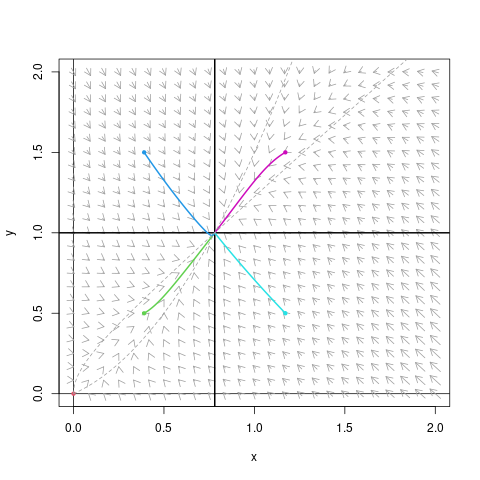
\includegraphics[width=.5\textwidth]{DynPopMaleFemelleCouple.png}
  $$
  }
\end{enumerate}



%-------------------------------------------------------------------------------
\subsubsection{Chemostat}
%-------------------------------------------------------------------------------

Voir \url{https://umr5558-shiny.univ-lyon1.fr/web/}


